\documentclass{standalone}
%\documentclass[a4paper,10pt]{scrartcl}

\usepackage[utf8]{inputenc}
\usepackage{tikz}
\usetikzlibrary{fit}

\begin{document}

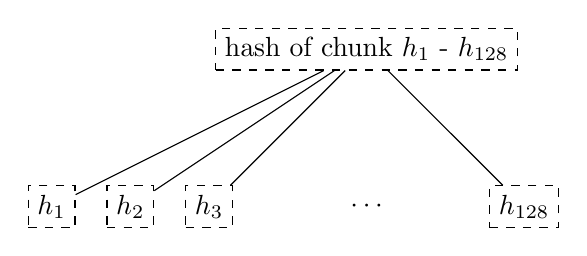
\begin{tikzpicture}
\node[draw,dashed] (root) at (5,3) {hash of chunk $h_1$ - $h_{128}$};
\node[draw,dashed] (h1) at (1,1) {$h_1$};
\node[draw,dashed] (h2) at (2,1) {$h_2$};
\node[draw,dashed] (h3) at (3,1) {$h_3$};
\node (dots) at (5,1) {$\cdots$};
\node[draw,dashed] (h128) at (7,1) {$h_{128}$};
% \node[draw,fit=(h1) (h2) (h3) (dots) (h128)]{};
\draw (root) -- (h1);
\draw (root) -- (h2);
\draw (root) -- (h3);
\draw (root) -- (h128);
\end{tikzpicture}
\end{document}
